
\documentclass[12pt,letterpaper]{article}
\usepackage{pset-2023}


\qa{q} % a="answers only"; q ="questions only"; b="both"
\usepackage{qa}

%figuring out points per question: quiz component currently at 28 points
%so need 72 points for part II, over eight subquestions. so avg 9 points per subquestion 

%other question ideas: have them discuss whether they think the control hypothesis is correct or not. 


\begin{document}


\psintro{Problem Set 4: Time Travel}


%\fbox{\parbox{150mm}{\emph{Warning:} At this point, you're doing philosophy. Keep in mind that even if a problem is murky, it can be addressed in more or less thoughtful ways: a good answer will reveal that you've understood the complexity of the underlying terrain and that you've given the issue serious thought.}



\subsection*{Part I (28 points; answer on Canvas Quiz for this part)} 



\begin{enumerate}


\item \question{Recall that for a time-travel story to be consistent, it must never give us conflicting descriptions of a single point in the narrative's timeline.

With that in mind, determine whether each of the the following stories can be interpreted as a consistent time travel story. (Make sure you interpret them as stories about ordinary time, rather than super-time, and that you interpret them as time travel stories rather than world-travel stories.)}

\begin{enumerate}






\item \question{After doing badly in an exam, you resolve to travel back in time to give yourself a hint before the exam takes place. You successfully travel back in time but mistakenly hand your earlier self the wrong hint and end up doing even worse on the exam. (2~points)}

\answer{This is an inconsistent time travel story. At the beginning of the story you are told that you do poorly on an exam; at the end of the story you are told that you do even worse than that.}



\item \question{In your youth, you discover plans to build a time-machine under your bed. You successfully build a time machine, only to discover that time travel isn't really to your liking. The past is much too dangerous and the future much too warm. So you decide to destroy your time machine. Just to be on the safe side, you use it one last time to travel back in time, and you destroy the plans that are lying under your bed, before your younger self has a chance to look at them. (2~points)}

\answer{This is an inconsistent time travel story. At the beginning of the story you are told that your younger self finds the plans under the pillow; at the end of the story you are told that the plans are destroyed before your younger self has a chance to see them.}


\item \question{As a child, Oscar goes for a walk in the forest. For a few seconds, he experiences the odd sensation of being watched. Many years later, he uses a time machine to travel back to that fateful day. He finds a good hiding place in the forest and spends a few seconds watching his younger self. As an old man, he again uses a time machine to travel back to that fateful day. He finds an even better hiding place and---like a champion creep---spends a few seconds watching his middle-aged self watch his younger self. (2~points)}

\answer{This is a consistent time travel story.}

\item \question{A team of lepidopterists travels back in time to the Paleogene, hoping to catch a glimpse of early butterflies. The team is cautioned not to interfere with the past in any way. But accidents happen. As they are completing their journey, one of the scientists steps on a branch and startles a butterfly. When the team returns to the present, they are confronted with changed world. Land octopuses have conquered the Earth and rule with an iron tentacle. A small interference in the past has made a big difference to the future. (2 points)}

\answer{This is an inconsistent time travel story. The beginning of the story presupposes that the present day is one way; the end of the story tells us that the present day is ``changed'' with respect to that, with land octopuses ruling the world. }

\item \question{At time $t$ you wake up to find plans for building a time machine in your desk drawer. You use the plans to build a time machine, and spend many happy years traveling through time. During one of your travels you go back to time $t$ and leave the plans in your younger self's desk drawer. (2 points)}

\answer{This is a consistent time travel story. (It does involve causal loops: the presence of the plans under your pillow causes you to travel in time, which causes the presence of the plans under your pillow. This makes the story weird. But weirdness is not the same as inconsistency.)

}

\end{enumerate}

\item[2.--7.] See \textbf{additional six questions} (\#2--\#7) on Canvas Quiz for Part I (18 points)!

\answer{Answers are indicated in the Canvas Quiz, along with occasional explanations for wrong answers. Let Hunt know if you need more details!}


\end{enumerate}



%%%%%%
%PART II
%%%%%%
%\newpage
\subsection*{Part II (72 points; justify all answers, preferably typed!)} 
\begin{enumerate}
\setcounter{enumi}{7}





\item \question{Recall the Control Hypothesis:

\begin{description}
\item[Control Hypothesis]
An agent acts freely in doing $X$ if and only if: (1) she does $X$ by making a certain decision, and (2) she is in a position to do something other than $X$ by making a different decision.
\end{description}
Now consider the following scenarios:}



\begin{enumerate}

\item \question{\begin{quote}Felix is on his way to the bookstore to buy a book. You know him well enough to know that he only likes to read detective stories. So you know from the start that he will choose a detective story. And sure enough: he leaves the bookstore with a detective story, even though he was in a position to choose any book he wanted.
\end{quote}

According to the Control Hypothesis, did Felix act freely in choosing a detective story? Keep in mind that you were able to predict that he would pick a detective story from the start. (6 points; don't forget to justify your answer)}

\answer{Yes, since we are explicitly told that he was in a position to choose any book he wanted.}

\vspace{3mm}
\item \question{\begin{quote}Bruno is on his way to kill Grandfather. You know that Grandfather is Bruno's grandfather.\footnote{Also, you know that there is no funny business: no rising up from the dead, no frozen sperm, no replicated DNA, etc.} So you know from the start that Bruno will fail. And sure enough: Bruno has a change of heart at the last minute and decides to put down the gun, even though he was in a position to make a different decision and pull the trigger instead.
\end{quote}
According to the Control Hypothesis, did Bruno act freely in putting down his gun? Keep in mind that you were able to predict that he wouldn't kill Grandfather from the start. (6 points; don't forget to justify your answer)}

\answer{Yes. We are explicitly told that Bruno decided to put down the gun even though he was in a position to decide differently and pull the trigger. And that's what it takes to act freely, according to the Control Hypothesis. 


}

\vspace{3mm}
\item

\question{
	\begin{quote}
After an hour of good fun, you decide to leave the party early and spend the rest of the evening at home. Unbeknownst to you, your hosts were finding you a bit tedious, so they were about to ask you to leave just as you left. So, had you instead decided to stay a little longer, you wouldn't have been able to: you would have been forced to leave early anyway. 
\end{quote}
According to the Control Hypothesis, did you act freely in leaving the party early? Is that answer intuitively correct?} (10 points)


\answer{You would have left the party even if you had made a different decision. So the Control Hypothesis entails that you did not act freely in leaving the party early. This is the wrong result intuitively, since your departure was caused by your decision to leave, with no external interference. 
}



\end{enumerate}

%\newpage

%\com{
\item \question{Describe how you could use a time machine to give yourself an extension on this problem-set, in a logically consistent manner. Assume that you get the time machine on Sunday 3/12/23, that the problem set remains due on Sunday 3/19/23, that Hunt will NEVER give an extension, and that the TAs are not suckers and cannot be bought off. Be careful out there! (10 points)}
% (Alternatively, if you think it's not possible to give yourself an extension, explain why not)
%As far as you know, you have never interacted with yourself in the past, and no one has any reports of you in the past. 

\answer{Here's one way: you get the time machine on Sunday 3/12/23. You travel forward to Monday and spend the day working on the pset in complete isolation from humanity. You then travel back in time with your answers. You go through Monday normally (while your personal-time past self is busily working away!). By spending as much time in the future (or past) as you like, you could obtain an arbitrarily large extension. You could even travel to the same time on multiple occasions, leading to multiple time-slices of yourself working away simultaneously.

Note that you could also travel to the past. If you do travel to the past, then it is true right now that some version of you was working away on a problem-set at some point in the past. Since this would already by true now, it would be impossible for you to change the past and thereby `butterfly effect' any problems. Of course, no one now presumably has any record of our students working on PSet 3 before 3/12/23, so the student's story has to be consistent with this.}

%}



\item \question{Very roughly, to \textit{causally explain} (or `mechanistically explain') how event $x$ occurs (or why it occurs) is to describe a (continuous) sequence of causes and effects leading to $x$'s occurrence, where causes strictly precede their effects in time (assume causation is temporally asymmetric). Consider the following scenario:}

\begin{enumerate}
%\com{ %left out in 2022 version 
\item[] \question{\begin{quote}On your 21st birthday, an elderly stranger hands you a nautically themed clock. The clock is strikingly beautiful---mesmerizing even, with its moving boats and cuttlefish (we LOVE cuttlefish). Many years later, in your old age, you travel back in time to your 21st birthday and hand the clock to your younger self.
\end{quote}

\vspace{1.5mm}

In this scenario, is there a {causal explanation} to be given about how the clock was originally built? If so, spell it out. If not, explain why not. (10 points)
}

\answer{No, there is no causal explanation to be given. For there is no sequence of events that causes the clock to be built. Instead, its presence, fully formed, at any given time is caused by its presence, fully formed, at some other time. For instance, its presence, fully formed, at the time of your 21st birthday is caused by its presence, fully formed, in your time machine many years later, which is in turn caused by your having received the clock, fully formed, on your 21st birthday.}

\vspace{3mm}
%}

\com{ %left out in 2023 version 
\item \question{\begin{quote}Olivia travels to the past in an effort to kill her grandfather before he has any children. On pain of contradiction, Olivia will fail to kill Grandfather.\footnote{As usual, we are assuming no funny business: no rising up from
the dead, no frozen sperm, no replicated DNA, etc.}\end{quote}

Extend the story so that it entails a causal explanation of why Olivia fails to kill Grandfather. (10 points)}

\answer{A good answer might look something like this:

\begin{quote}
The portion of the story detailed in the problem set does not settle the question of why Olivia does not succeed. But here is one way of spelling out the story that does: a dog barks, Olivia gets distracted, aims a little too far to the right, and the bullet ends up flying past Grandfather's left cheek. On this way of spelling out the details, a causal explanation for why Olivia does not succeed can be given as follows: a barking dog caused Olivia to get distracted, which caused her to aimed a little too far to the right, which caused her to miss.
\end{quote}
}
}




\end{enumerate}


\item \question{Consider the following scenario:

\begin{quote}You're wondering whether to study for tomorrow's biology exam. It's a hard exam and you won't pass unless you study. Just then you see your good friend Amy emerge from a time machine. She announces that she's been to the future and has seen you pass the exam. Amy is totally reliable, so you can be 100\% confident that you will pass the exam. 
\end{quote}
Does this scenario entail that you'll pass even if you don't study? (10 points; don't forget to justify your answer.)}

\answer{No. It's an explicit part of the story that you won't pass unless you study. So we may conclude from the fact that you will, in fact, pass the exam that you will, somehow or other, study. Ideally, a student would convey understanding that determinism does not entail fatalism. Even though the past determines that you will do well on the exam, this isn't the case \textit{no matter what happens}. It is not fatalistically the case that you will do well, i.e. do well no matter what you do.}

%(A ``yes'' answer could in principle get credit, if it's sufficiently justified.)}


\com{
\item \question{On April 2, 2023, Bruno enters a time machine to travel to December 31st, 1999. In eager anticipation of his journey, Bruno says ``Soon I will witness the turn of the millennium.'' Use the distinction between personal time and external time to explain how Bruno's statement can be interpreted as a consistent statement. (3 points)}
} %end com 

\com{
\item \question{The course materials describe a toy model of time travel. The diagram below depicts a wormhole within the world of the toy model. The points represented by \emph{W-} are identified with the points represented by \emph{W+}. Particle $A$ jumps to the future when its spacetime trajectory reaches the wormhole from outside the wormhole region; particle $B$ jumps to the past when its spacetime trajectory reaches the wormhole from inside the wormhole region.


\begin{center}
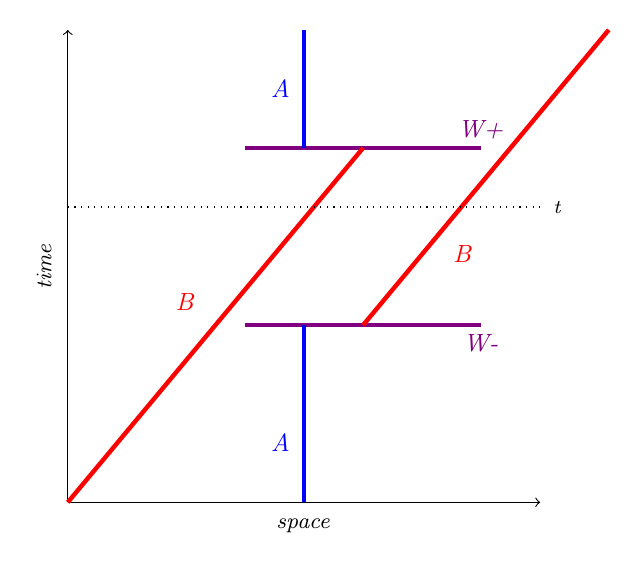
\begin{tikzpicture}[scale = 0.75]
\draw[->] (0,0) -- (0,8); % time axis
\draw[->] (0,0) -- (8,0); % space axis
\node at (4,-0.4) {\footnotesize \emph{space}}; % space label
\node at (-0.4,4) {\footnotesize \rotatebox{90}{\emph{time}}}; % time label

\draw[ultra thick, violet] (3,6) -- (7,6); % Line W+
\node[violet] at (7,6.3) {\small \emph{W+}}; % W+'s label
\draw[ultra thick, violet] (3,3) -- (7,3); % Line W-
\node[violet] at (7,2.7) {\small \emph{W-}}; % W-'s label

\draw[ultra thick, blue] (4,0) -- (4,3); % A's timeline, part 1
\node[blue] at (3.6,1) {\small \emph{A}}; % A's label, part 1
\draw[ultra thick, blue] (4,6) -- (4,8); % A's timeline, part 2
\node[blue] at (3.6,7) {\small \emph{A}}; % A's label, part 2
%\node at (4,3.3) {\footnotesize $p$}; % p label
%\node at (4,5.7) {\footnotesize $p$}; % p label


\draw[ultra thick, red] (0,0) -- (5,6); % B's timeline, part 1
\node[red] at (2,3.4) {\small \emph{B}}; % B's label, part 1
\draw[ultra thick, red] (5,3) -- (9.16,8); % B's timeline, part 2
\node[red] at (6.7,4.2) {\small \emph{B}}; % B's label, part 2
%\node at (6,6.4) {\footnotesize $p'$}; % p label
%\node at (6,2.6) {\footnotesize $p'$}; % p label

\draw[dotted] (0,5) -- (8,5); % time t line
\node[black] at (8.3,5) {\scriptsize \emph{t}}; % time t label

%\draw[dotted] (0,1.7) -- (8,1.7); % time t line
%\node[black] at (8.3,1.7) {\scriptsize \emph{t}}; % time t label
%
%\draw[dotted] (0,5.2) -- (8,5.2); % time t line
%\node[black] at (8.3,5.2) {\scriptsize \emph{t$'$}}; % time t label


\end{tikzpicture}
\end{center}
Note that only one particle---particle $B$---exists at time $t$, though $B$ experiences time $t$ twice. 

Now consider a different diagram:

\begin{center}
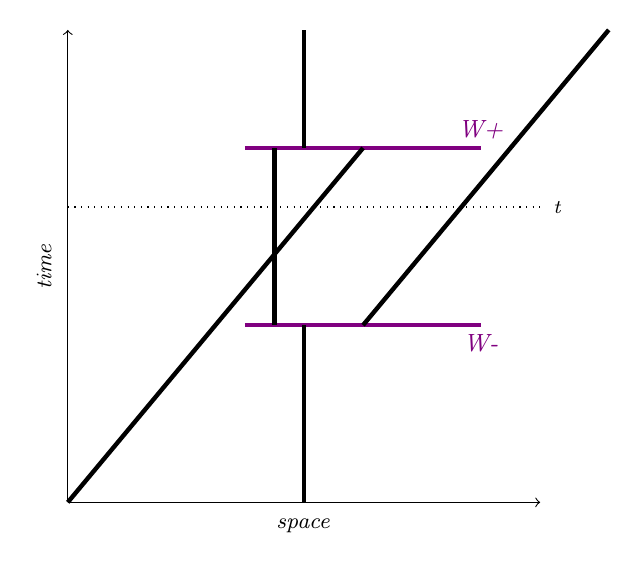
\begin{tikzpicture}[scale = 0.75]
\draw[->] (0,0) -- (0,8); % time axis
\draw[->] (0,0) -- (8,0); % space axis
\node at (4,-0.4) {\footnotesize \emph{space}}; % space label
\node at (-0.4,4) {\footnotesize \rotatebox{90}{\emph{time}}}; % time label

\draw[ultra thick, violet] (3,6) -- (7,6); % Line W+
\node[violet] at (7,6.3) {\small \emph{W+}}; % W+'s label
\draw[ultra thick, violet] (3,3) -- (7,3); % Line W-
\node[violet] at (7,2.7) {\small \emph{W-}}; % W-'s label

\draw[ultra thick] (4,0) -- (4,3); % A's timeline, part 1
%\node[blue] at (3.6,1) {\small \emph{A}}; % A's label, part 1
\draw[ultra thick] (4,6) -- (4,8); % A's timeline, part 2
%\node[blue] at (3.6,7) {\small \emph{A}}; % A's label, part 2


\draw[ultra thick] (0,0) -- (5,6); % B's timeline, part 1
%\node[red] at (2,3.4) {\small \emph{B}}; % B's label, part 1
\draw[ultra thick] (5,3) -- (9.16,8); % B's timeline, part 2
%\node[red] at (6.7,4.2) {\small \emph{B}}; % B's label, part 2

\draw[ultra thick] (3.5,3) -- (3.5,6); % C's timeline

\draw[dotted] (0,5) -- (8,5); % time t line
\node[black] at (8.3,5) {\scriptsize \emph{t}}; % time t label


\end{tikzpicture}
\end{center}
Assuming the laws of the toy model are in place, how many different particles exist at time $t$? (8~points; don't forget to explain your answer)
}

\answer{One. But three different time-slices of that one particle occur at three different locations at time $t$. 

To see this, consider the particle corresponding to the left-most spacetime trajectory in the diagram. It starts out moving right. After a while, it enters the wormhole region and collides with an later version of itself, which is stationary. The collision causes it to become stationary. While stationary it reaches time $t$. It then reaches the wormhole and jumps to the past. After a while it collides with an earlier version of itself, which is moving right. The collision causes it to start moving right again. While moving right, it reaches time $t$ a second time. After that, it reaches the wormhole a second time and again jumps to the past. It continues moving right and reaches time $t$ for a third time. Shortly after that, it exits the spacetime region.}
} %end com 


\item \question{There is a famous scene in the film \emph{The Matrix} in which the Oracle predicts that Neo will break a vase. (You can find it online by searching ``matrix oracle vase".\footnote{Or you can go here: \url{https://www.youtube.com/watch?v=eVF4kebiks4}}) }

\begin{enumerate}
\item \label{neo-a}
\question{Describe a consistent time travel story that uses time travel to explain how the Oracle acquires the information necessary to issue her successful prediction. \\ (10 points)}

\answer{One possible answer might look like this:

\begin{quote}
Before Neo's visit, the Oracle travels to the future and witnesses the visit from a hidden location. She sees her (personal-time) future self warn Neo about the vase, and sees Neo turn around and break it. She then travels back to the past and uses this information in deciding what to say during Neo's visit.
\end{quote}
Other stories are possible, of course, but only students who give consistent time travel stories should be given full credit.
}

\item \question{Neo breaks the vase after turning partially around. Does the Control Hypothesis entail that, according to the story you gave in your response to (\ref{neo-a}), Neo fails to act freely in turning around? (10 points)}

\answer{The Control Hypothesis does not entail that, according to the story above, Neo fails to act freely in turning around. For the story says nothing to rule out that Neo turns around by deciding to turn around, and it says nothing about what would have happened had Neo decided differently. \\ Note that based on our discussion in class (or lecture slides), the student might also discuss the Weak Principle of Alternative Possibilities (Weak PAP). For all we know, if Neo had wanted to act differently, then he could have. E.g. if he hadn't wanted to turn around, then he wouldn't have. If this is the case, then Neo would have acted freely according to the Weak PAP.}

\end{enumerate}


%left out for variety in 2022-23
\com{
\item \question{Bruno travels back in time to kill his grandfather, to a time before his grandfather
had any children. Will he succeed? (Assume no funny business: no rising up from
the dead, no frozen sperm, no replicated DNA, etc.) (20 points)

\begin{itemize}
\item If you think the answer is ``yes'', tell a consistent story that makes clear how it is that Bruno succeeds.

\item If you think the answer is ``no", tell a consistent story that makes clear why Bruno does not succeed.


\end{itemize}
}


\answer{A good answer might look something like this:

\begin{quote}
No, he will not succeed. For the assumption that he succeeds makes the story inconsistent: we are told, on the one hand, that Grandfather is a grandfather (and therefore survives long enough to have children), and, on the other,  that Grandfather is killed before he has any children.

The portion of the story detailed in the problem set does not settle the question of why Bruno does not succeed. But here is one way of spelling out the story that does: Bruno aims a little too far to the right, and the bullet ends up flying past Grandfather's left cheek. On this way of spelling out the details, the reason why Bruno does not succeed is that he aimed a little too far to the right.
\end{quote}
}
}





\end{enumerate}

\end{document}


\question{
\subsection*{Optional:}

Is contemporary physics compatible with time travel? Alan Guth, who is a famous physicist at MIT, tackled this question during a visit to \emph{Paradox and Infinity}, a few years ago. You can check out his lecture here: 
\begin{center}
  \includegraphics[width=2.9cm]{guthqrcode.png}\\
\url{bit.ly/2ToPthV}
\end{center}


}





